% This work by Jeremy A. Hansen is licensed under a Creative Commons 
% Attribution-NonCommercial-ShareAlike 3.0 Unported License, 
% as described at http://creativecommons.org/licenses/by-nc-sa/3.0/legalcode

%Conditionals

Conditionals are used to direct the program to different sections of code. 
In plain English, we might have a statement ``If X is greater than Y, do this...'' Conditionals direct the program to behave differently depending on the results of a comparison. Several common comparison operators used in C++ are:

\begin{table}[bh]
	\centering
		\begin{tabular}{| c | p{3.5in} |}
		\hline
			\textbf{Symbol} & \textbf{Meaning} \\ \hline
			\Code{==} & Is equal to \\ \hline
			\Code{!=} & Is not equal to \\ \hline
			\Code{>=} &	Greater than or equal to \\ \hline
			\Code{<=} &	Less than or equal to \\ \hline
			\Code{>} &	Greater than \\ \hline
			\Code{<} &	Less than \\ \hline
			\Code{\&\&}, \Code{and} &	Logical AND: The condition on the left \emph{AND} the condition on the right must be true \\ \hline
			\Code{||}, \Code{or} &	Logical OR: The condition on the left \emph{OR} the condition on the right must be true \\ \hline
		\end{tabular}
  \caption{Common comparison operators}
\end{table}

\LevelD{\Code{if}, \Code{else}, and \Code{else if}}

The most popular conditional is the \Code{if} statement. 
An \Code{if} statement looks like this: \nopagebreak[4]

\noindent\begin{minipage}{\linewidth}\begin{lstlisting}
if(variable == variable2)
{
  // Code here executes only when
  // the value of variable is the same as variable2
}
\end{lstlisting}\end{minipage}

The keyword \Code{if} is used to start the statement. 
Parentheses are used to contain the conditional expression. 
If the expression inside the parentheses is true, then the following expression will be executed.

\LevelE{A small digression on expressions}

Note that curly braces merely surround expressions to become a single expression.
The act of surrounding expressions creates a code block.
However, having only one expression within a code block is the same as not having it in a code block.

\noindent\begin{minipage}{\linewidth}\begin{lstlisting}
if (variable == variable2)
{
  cout << "Yes!";
}
\end{lstlisting}\end{minipage}

\noindent is the same as

\noindent\begin{minipage}{\linewidth}\begin{lstlisting}
if (variable == variable2)
  cout << "Yes!";
\end{lstlisting}\end{minipage}

It is not recommended to go without braces for mere brevity at the cost of making mistakes later on.

For example, suppose you have some code for baking bread, like the following.

\noindent\begin{minipage}{\linewidth}\begin{lstlisting}
if (breadType == 10)
  ovenFanOn = true;
\end{lstlisting}\end{minipage}

But then later you are told that bread type 10 needs to be cooked at $350^{\circ}F$.
So you make the following change:

\noindent\begin{minipage}{\linewidth}\begin{lstlisting}
if (breadType == 10)
  ovenFanOn = true;
  ovenTemp = 350;
\end{lstlisting}\end{minipage}

Except.. that is really the same as.. 

\noindent\begin{minipage}{\linewidth}\begin{lstlisting}
if (breadType == 10)
  ovenFanOn = true;

ovenTemp = 350;
\end{lstlisting}\end{minipage}

So now the baker is mad because every bread is being cooked wrong except bread type 10!
What you really meant was: 

\noindent\begin{minipage}{\linewidth}\begin{lstlisting}
if (breadType == 10)
{
  ovenFanOn = true;
  ovenTemp = 350;
}
\end{lstlisting}\end{minipage}

Here's another bear trap that you'll likely hit:

\noindent\begin{minipage}{\linewidth}\begin{lstlisting}
if (breadType == 9);
  ovenFanOn = true;
\end{lstlisting}\end{minipage}

It is still valid syntax, but the expression after the \Code{if} statement is an empty expression.
An empty expression does nothing, and so now every bread type will have the fan on, which is not what the baker wanted.


\LevelE{Using \Code{else}}


\begin{figure}[tbh]
  \centering
  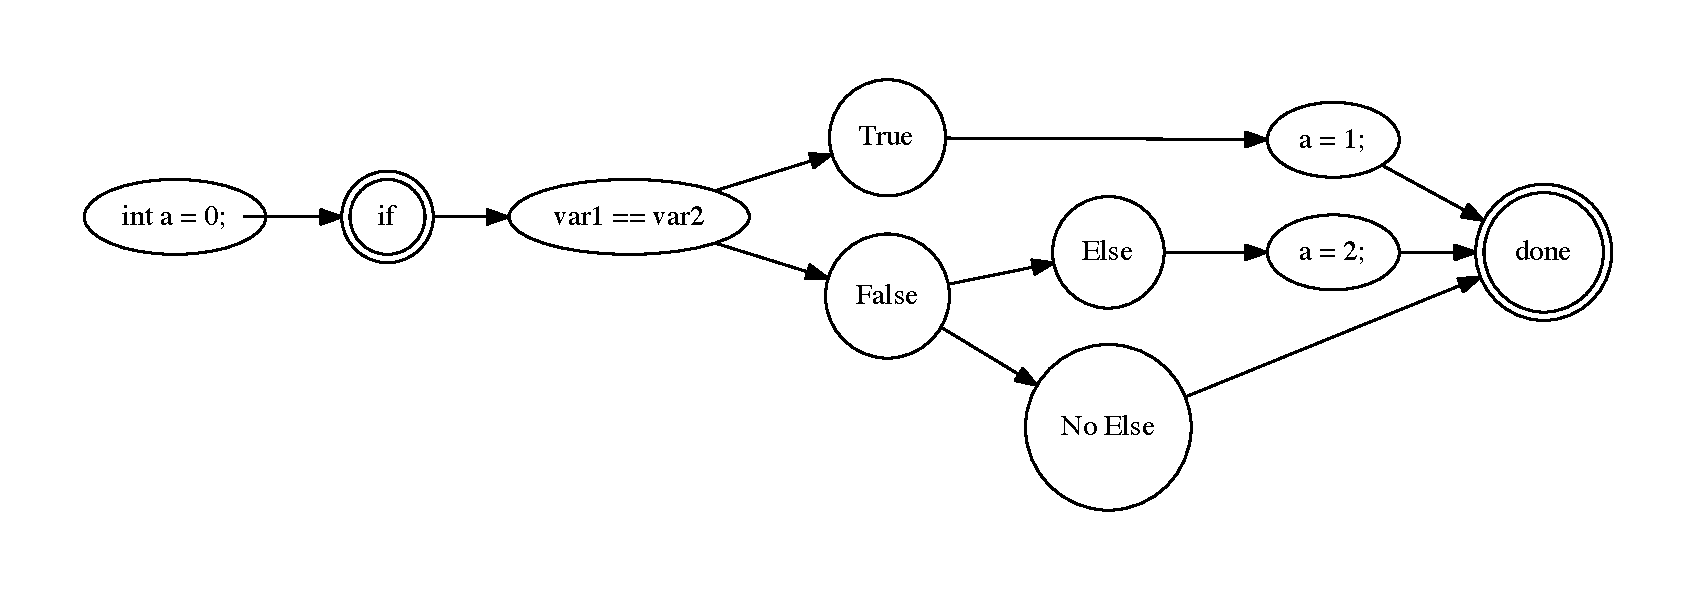
\includegraphics[width=\textwidth]{diagrams/if-flow.pdf}
  \caption{\Code{if} and \Code{else} statement flow of execution} \label{fig-if-flowchart}
\end{figure}


An \Code{else} statement may be placed after an \Code{if} statement, and any time the expression inside the parentheses following the \Code{if} is not true, the code inside the \Code{else} block is executed. 
For example:

\noindent\begin{minipage}{\linewidth}\begin{lstlisting}
int a = 0;
if(var1 == var2)
{
  // Code here executes only when
  // the value of variable is the same as variable2
  a = 1;
}
else
{
  // Code here executes if they are not the same
  a = 2;
}
\end{lstlisting}\end{minipage}

An \Code{else} statement is used when you want some code to execute in any other case where the \Code{if} statement is not true. 
An example of how this works is also shown in Figure \ref{fig-if-flowchart}.

% \label{fig-else-flowchart}

An \Code{else if} could also be placed after the \Code{if} statement. 
An \Code{else if} is an additional \Code{if} statement checked only when the previous \Code{if} statement is false. 
While \Code{else} is a catch-all, \Code{else if} chains an \Code{if} to test for other conditions. 
Multiple \Code{else if} statements can be used, and they are all checked sequentially, and if necessary, an \Code{else} statement can be included at the end as a final catch-all. 
Take a look at Figure \ref{fig-else-if-flowchart} for a flowchart example.

% ^ I (Levi) personally think this is being taught wrong.



\begin{figure}[tbh]
  \centering
  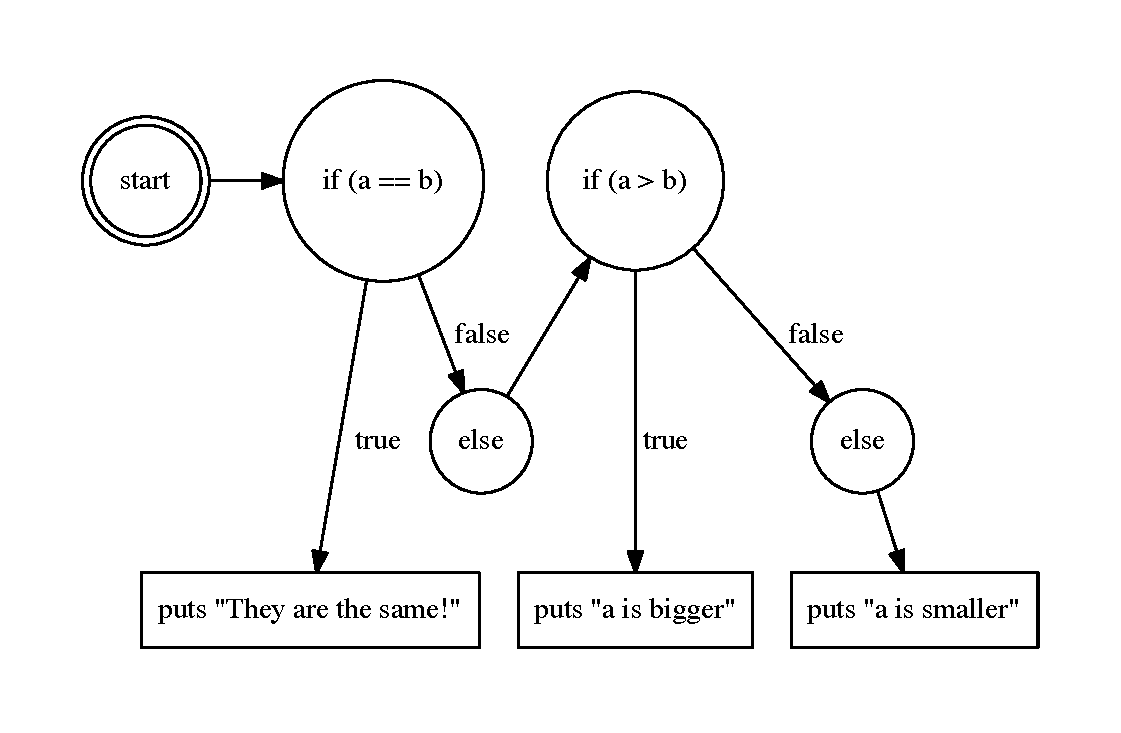
\includegraphics[width=\textwidth]{diagrams/if-else.pdf}
  \caption{How \Code{if}-\Code{else} chaining works} \label{fig-else-if-flowchart}
\end{figure}

Here's what the three statements would look like all together: \nopagebreak[4]

\noindent\begin{minipage}{\linewidth}\begin{lstlisting}
if(a == b)
{
  cout << "They are the same!" << endl;
}
else if(a > b)
{
  cout << "a is bigger!" << endl;
}
else
{
  cout << "a is smaller!" << endl;
}
\end{lstlisting}\end{minipage}

Note that every conditional expression is in parentheses.
Each \Code{if} must be followed by a \Code{(...)} in C++. 
Conditional expressions also appear in loops (discussed in Chapter \ref{chap_loops}) and \Code{switch} statements.

\LevelD{\Code{switch} statements}

\Code{switch} statements (also sometimes called \Code{switch}-\Code{case} statements) make a menu-like set of blocks. 
It does the same job as many \Code{if} statements, but can simplify the job when used correctly. 
Here is an example:

\noindent\begin{minipage}{\linewidth}\begin{lstlisting}
switch(variable):
{
  case 1:
    //code to execute when variable is equal to 1
    break;
  case 2:
    //code to execute when variable is equal to 2
    break;
  default:
    //code to execute when variable is neither 1 nor 2
    break;
}
// Resume here after a break
\end{lstlisting}\end{minipage}

If \Code{variable} is equal to 1 then the code following \Code{case 1:} will be executed.
If it is equal to 2, then the code following \Code{case 2:} will be executed, and if it is equal to neither, then the code following \Code{default:} will be executed. 
The cases are separated by the \Code{break} statement, which forces the code to leave the \Code{switch} statement's block of code. This code: \nopagebreak[4]

\noindent\begin{minipage}{\linewidth}\begin{lstlisting}
switch(variable)
{
  case 1:
    cout << "You picked case 1. Lame.";
    break;

  case 2:
    cout << "Case two is way better.";
    break;

  default:
    cout << "WRONG!";
    break;
}
\end{lstlisting}\end{minipage}

\noindent is equivalent to this code: \nopagebreak[4]

\noindent\begin{minipage}{\linewidth}\begin{lstlisting}
if (variable == 1)
{
  cout <<  "You picked case 1. Lame.";
}
else if (variable == 2)
{
  cout << "Case two is way better.";
}
else
{
  cout << "WRONG!";
}
\end{lstlisting}\end{minipage}

When there are only a few cases, \Code{if}, \Code{else if}, and \Code{else} statements are often easier. 
However, when you get to a greater number of cases, \Code{switch} statements become easier.

In \Code{switch} statements, only one \Code{case}'s code executes, provided that each \Code{case} is followed by \Code{break}. 
Otherwise, the program continues execution until it reaches a \Code{break} statement or the end of the \Code{switch} block. 
With an \Code{if} and \Code{else if}, only one branch may be executed, but the conditions in each \Code{if} are evaluated.

\begin{table}[bh]
		\begin{tabular}{| p{1.5in} | p{2.5in} |}
		\hline
			\textbf{User enters} & \textbf{Output} \\ \hline
			\Code{//Program start} &	<1> Addition \newline				<2> Subtraction\newline				             <3> Compare\newline							Type the number of your desired option: \\ \hline
			\Code{1} & The result of this addition is 9.3 \\ \hline
			\Code{2} & The result of this subtraction is 0.9 \\ \hline
			\Code{3} & A is greater than B \\ \hline
			\Code{//anything other than 1, 2, or 3} &	Not an option \\ \hline
		\end{tabular}
  \caption{The sample program's output}
  \label{table-conditional-program}
\end{table}


Here is some code that uses both \Code{switch} and \Code{if} statements.
Compiling and running the following code results in the output in Table \ref{table-conditional-program}.

\noindent\begin{minipage}{\linewidth}\begin{lstlisting}
#include <iostream>
using namespace std;
int main()
{
  int choice;
  double a = 5.1, b = 4.2;

  cout << "<1> Addition\n";
  cout << "<2> Subtraction\n";
  cout << "<3> Compare\n";

  cout << "Type the number of your desired option:\t";
  cin >> choice;

  switch(choice)
  {
    case 1:
	    cout << "The result of this addition is " 
	      << a + b << endl << endl;
	    break;

    case 2:
	    cout << "The result of this subtraction is "
	      << a - b << endl << endl;
	    break;

    case 3:
      if (a > b)
		    cout << "A is greater than B";
      else if (a < b)
		    cout << "A is less than B";
	    else //a == b
		    cout << "A equals B";
	    break;

    default:
      cout << "Not an option";
      break;
  }

  return 0;
}
\end{lstlisting}\end{minipage}








\LevelD{Review Questions}
\begin{enumerate}
\item What is the output of the following code?

\noindent\begin{minipage}{\linewidth}\begin{lstlisting}
int a = 5;
int b = 10;

if(a > b)
  cout << "a is greater than b.";
else
  cout << "b is greater than a.";
\end{lstlisting}\end{minipage}

\item Why are \Code{switch} statements useful?

\item When are braces (\Code{\{\}}) needed in an \Code{if} statement?

\item Write a program that checks which number is higher than another and prints out an appropriate message. This program should use 2 variables, an \Code{if} statement and an \Code{else} statement. Bonus: Rewrite it to also check if the numbers are equal.

\end{enumerate}

\LevelD{Review Answers}

\begin{enumerate}
\item \Code{b is greater than a.}
\item \Code{switch} statements are useful for making menus for the user. (Other answers are also possible)
\item Braces are needed for any code longer than 2 lines following an \Code{if}.
\item \noindent\begin{minipage}{\linewidth}\begin{lstlisting}
#include <iostream>
using namespace std;
int main()
{
  int input1, input2;
  cout << "enter a number: ";
  cin >> input1;
  cout << "enter a number to compare to the first: ";
  cin >> input2;
  if(input1 > input2)
    cout << input1 << " is greater than " << input2;
  else
    cout << input2 << " is greater than " << input1;
}
\end{lstlisting}\end{minipage}

\end{enumerate}

%\LevelD{Further Reading}
%
%\begin{itemize}
%\item ~
%\item ~
%\item ~
%\end{itemize}	

